\documentclass{beamer}
\usetheme{Madrid}
\usepackage{pifont}  % Подключаем пакет для использования \ding
\usepackage{tikz}
\usetikzlibrary{backgrounds}
\usepackage[table]{xcolor}
\usepackage{array}
\usepackage{graphicx}

\usepackage[english]{babel}  % Подключение для автоматического переноса слов





\title{Osint Bot Presentation}
\author{CEO | Yana Anisimova}

\begin{document}

\frame{\titlepage}

\section{What's the problem? Our people may be working for the enemy without even realizing it}

\begin{frame}
    \frametitle{What's the problem? Our people may be working for the enemy without even realizing it}
    
    \begin{block}{Questions that arise when applying for a job}
        \begin{itemize}
            \item Is the company I am going to work for connected to the aggressor country?
            \item Is it a reliable company?
            \item Is it worth getting involved?
            \item Will I have problems because I work or worked for this company?
            \item Etc.
            \item How can I quickly check an employer?
        \end{itemize}
    \end{block}
    
\end{frame}

\section{Our answer is Osint Bot}

\begin{frame}
    \frametitle{Our answer is Osint Bot}
    
    \begin{block}{AI-based Telegram bot that checks employer using OSINT methods}
        \begin{itemize}
            \item Find job postings of your employer on .ru and .by websites
            \item Analyze employer connections with the aggressor country using OSINT methods
        \end{itemize}
    \end{block}
    
\end{frame}

\section{It takes just 3 simple steps to get started:}

\begin{frame}
    \frametitle{It takes just 3 simple steps to get started:}
    
    \begin{block}{Enter company, enter job title. Get results}
        - Enter company name
        - Enter job title
        - Get rusult
    \end{block}
    
\end{frame}

\section{Market size: Ukrainian and Friends of Ukraine}

\begin{frame}
    \frametitle{Market size: Ukrainian and Friends of Ukraine}

    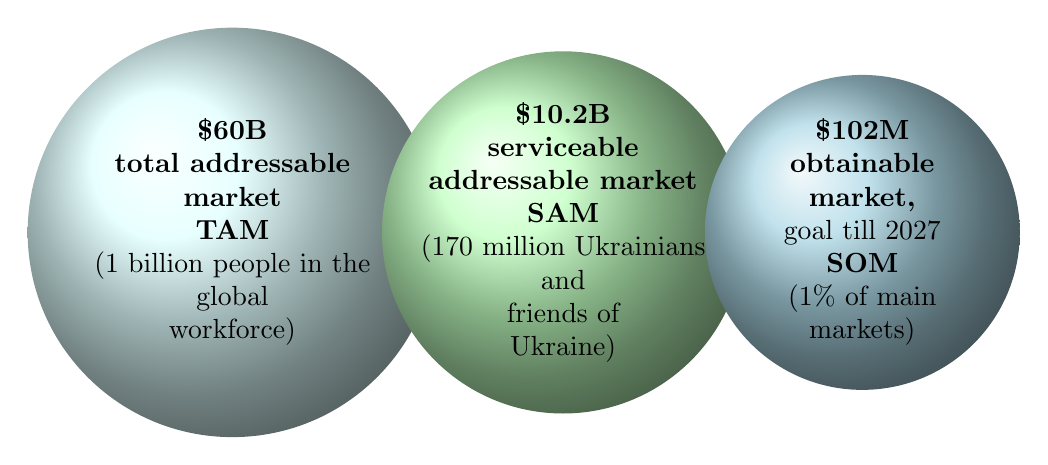
\begin{tikzpicture}

    % Colors for the circles
    \definecolor{lightblue}{RGB}{173,216,230}
    \definecolor{lightgreen}{RGB}{192,255,192}
    \definecolor{lightcyan}{RGB}{224,255,255}
    
    % TAM Circle
    \shade[ball color=lightcyan] (-11.7,0) circle (2.6cm);
    \node at (-11.7,0) {\parbox{4cm}{
        \centering
        \textbf{\$60B}\\
        \textbf{total addressable market}\\
        \textbf{TAM}\\
        (1 billion people in the global\\
        workforce)
    }};

    % SAM Circle
    \shade[ball color=lightgreen] (-7.5,0) circle (2.3cm);
    \node at (-7.5,0) {\parbox{4cm}{
        \centering
        \textbf{\$10.2B}\\
        \textbf{serviceable addressable market}\\
        \textbf{SAM}\\
        (170 million Ukrainians\\
        and\\
        friends of\\
        Ukraine)
    }};

    % SOM Circle
    \shade[ball color=lightblue] (-3.7,0) circle (2cm);
    \node at (-3.7,0) {\parbox{3cm}{
        \centering
        \textbf{\$102M}\\
        \textbf{obtainable market,}\\
        goal till 2027\\
        \textbf{SOM}\\
        (1\% of main markets)
    }};
    
    \end{tikzpicture}

\end{frame}


\section{How do we make money}

\begin{frame}
    \frametitle{How do we make money}
    
    \begin{tikzpicture}
        % Центрируем блоки на странице
        \node at (8,4.5) { % Центр альбомного слайда 16:9 (8 см, 4.5 см)
            \begin{tikzpicture}
                % First card
                \shade[left color=green!30, right color=blue!30, rounded corners] (0,0) rectangle (4.5,7);
                \draw[rounded corners, line width=1pt] (0,0) rectangle (4.5,7);
                \node[align=center, text width=4cm, font=\bfseries, anchor=north] at (2.25,6.5) {For free};
                \node[align=center, text width=4cm, font=\Large, anchor=north] at (2.25,5.5) {\$0/mo};
                \node[align=center, text width=4cm, font=\small] at (2.25,4) {The bot  \\ displays ads};
                
                % Second card (shifted by 6 cm to the right, which is width of the card + 1.5 cm gap)
                \shade[left color=green!30, right color=blue!30, rounded corners] (6,0) rectangle (10.5,7);
                \draw[rounded corners, line width=1pt] (6,0) rectangle (10.5,7);
                \node[align=center, text width=4cm, font=\bfseries, anchor=north] at (8.25,6.5) {Premium};
                \node[align=center, text width=4cm, font=\Large, anchor=north] at (8.25,5.5) {\$5/mo};
                \node[align=center, text width=4cm, font=\small] at (8.25,4) {Advanced features  \\ available};
            \end{tikzpicture}
        };
    \end{tikzpicture}
   
    
\end{frame}

    
   


\section{Competition}

\begin{frame}
    \frametitle{Competition}
    
   
    \begin{table}[ht]
        \centering
        \begin{tabular}{|>{\raggedright\arraybackslash}m{2cm}|>{\centering\arraybackslash}m{2.5cm}|>{\centering\arraybackslash}m{2.5cm}|>{\centering\arraybackslash}m{2.5cm}|}
        \hline
        \rowcolor{white} \textbf{Feature} & \textbf{\textcolor{orange}{Osint Bot}} & \textbf{Google} & \textbf{Chat GPT} \\
        \hline
        Available for telegram users & \cellcolor{green!10} Yes & \cellcolor{red!10} Additional registration required & \cellcolor{red!10} Additional registration required \\
        \hline
        No additional registration required & \cellcolor{green!10} Yes & \cellcolor{red!10} No & \cellcolor{red!10} No \\
        \hline
        Integrated with telegram & \cellcolor{green!10} Yes & \cellcolor{red!10} No & \cellcolor{red!10} No \\
        \hline
        Always at hand & \cellcolor{green!10} Yes & \cellcolor{red!10} No & \cellcolor{red!10} No \\
        \hline
        \end{tabular}
        \end{table}
        
        
            
   
    
\end{frame}

\section{Go to market strategy}

\begin{frame}
    \frametitle{Go to market strategy}
    
    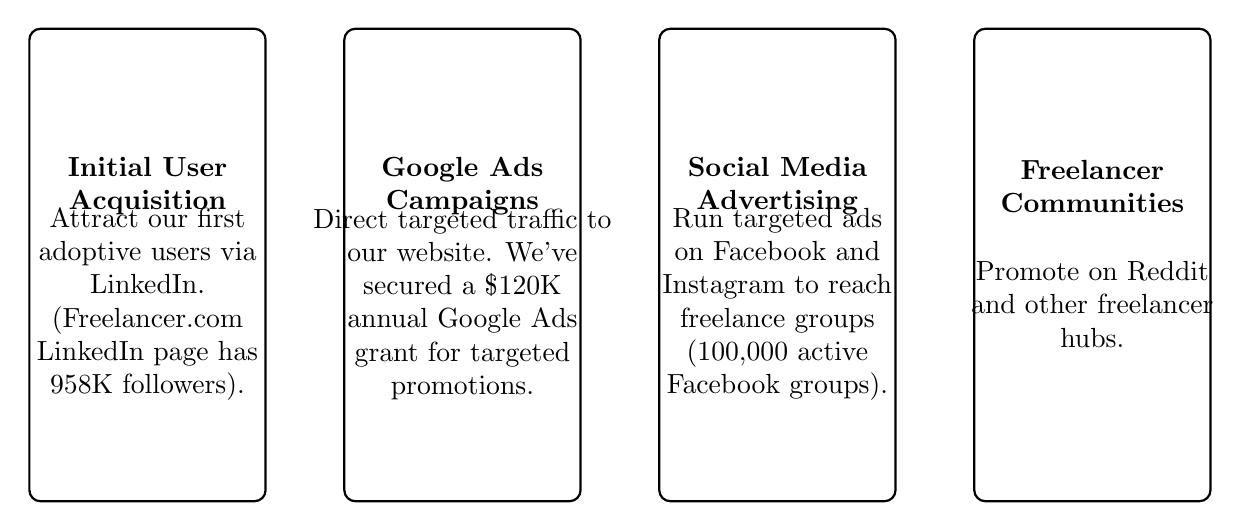
\begin{tikzpicture}

        % First Box: Initial User Acquisition
        \draw[rounded corners, thick] (0, 0) rectangle (3, -6);
        %\node at (1.5, -1) {\includegraphics[scale=0.2]{icon1.png}};
        \node[align=center] at (1.5, -2) {\textbf{Initial User}\\\textbf{Acquisition}};
        \node[align=center] at (1.5, -3.5) {Attract our first \\ adoptive users via \\ LinkedIn. \\
        (Freelancer.com \\ LinkedIn page has \\ 958K followers).};
        
        % Second Box: Google Ads Campaigns
        \draw[rounded corners, thick] (4, 0) rectangle (7, -6);
        %\node at (5.5, -1) {\includegraphics[scale=0.15]{icon2.png}};
        \node[align=center] at (5.5, -2) {\textbf{Google Ads} \\\textbf{Campaigns}};
        \node[align=center] at (5.5, -3.5) {Direct targeted traffic to \\ our website. We've \\ secured a \$120K \\ annual Google Ads \\ grant for targeted \\ promotions.};
        
        % Third Box: Social Media Advertising
        \draw[rounded corners, thick] (8, 0) rectangle (11, -6);
        %\node at (9.5, -1) {\includegraphics[scale=0.15]{icon3.png}};
        \node[align=center] at (9.5, -2) {\textbf{Social Media} \\\textbf{Advertising}};
        \node[align=center] at (9.5, -3.5) {Run targeted ads \\ on Facebook and \\ Instagram to reach \\ freelance groups \\ (100,000 active \\ Facebook groups).};
        
        % Fourth Box: Freelancer Communities
        \draw[rounded corners, thick] (12, 0) rectangle (15, -6);
        %\node at (13.5, -1) {\includegraphics[scale=0.15]{icon4.png}};
        \node[align=center] at (13.5, -2) {\textbf{Freelancer} \\\textbf{Communities}};
        \node[align=center] at (13.5, -3.5) {Promote on Reddit \\ and other freelancer \\ hubs.};
        
        \end{tikzpicture}
    
\end{frame}

\section{Our team}

\begin{frame}
    \frametitle{Our team}
    
    \begin{block}{}
        % Добавьте информацию о команде
        Yana Anisimova CEO 
        Yuriy Galych CTO
    \end{block}
    
\end{frame}

\section{Money raising}

\begin{frame}
    \frametitle{Money raising}
    
    \begin{block}{Money raising}
        % Добавьте описание стратегии привлечения средств
        \begin{itemize}
            \item Strategy 1
            \item Strategy 2
        \end{itemize}
    \end{block}
    
\end{frame}


\section{OSINT bot invites investors to join us for peace in Ukraine and Europe}

\begin{frame}
    \frametitle{OSINT bot invites investors to join us for peace in Ukraine and Europe}
    
    \begin{block}{Join us for peace in Ukraine and Europe}
        % Добавьте описание предложения для инвесторов
        \begin{itemize}
            \item Reason 1
            \item Reason 2
        \end{itemize}
    \end{block}
    
\end{frame}

\end{document}
